After the event selection (see Section~\ref{sec:event_selection}) the events are categorised based on the lepton multiplicity (1L or 2LOS), jets multiplicity and b-jets multiplicity. The two leptonic channels are analysed separately and combined only for the final results. 
In the 1L (2LOS) channel, events are retained for the final analysis if they contain at least 7 (5) jets and at least two $b$-tagged jets (a jet is considered as $b$-tagged if it passes an OP of 70\% efficiency). 
Signal-depleted and signal-rich analysis regions are defined from different combinations of jets and $b$-jets multiplicity requirements.  
An illustration of the used analysis regions is given in Figure~\ref{fig:regions}. The $b$-jets multiplicity requirements combine multiple $b$-tagging OP as described in Table~\ref{tab:regions}. The b-tagged jets are counted across different OPs using \textbf{AND} logic. The events in each category must fulfil all the three b-jets multiplicity requirements simultaneously. For example, in 3bH selection, an event should contain exactly three b-tagged jets obtained using b-tagging OPs with an average expected efficiencies of 60\%, exactly three b-tagged jets obtained using b-tagging OPs with an average expected efficiencies of 70\% and more than three b-tagged jets obtained using b-tagging OPs with an average expected efficiencies of 85\%.

\begin{table}[!hbt]
  \begin{center}
    \caption{
      Summary of the $b$-tagging requirements for the event categorisation.
      Events in each category must satisfy all requirements listed in columns.
      $N_b^{60\%}$, $N_b^{70\%}$ and $N_b^{85\%}$ are defined as the numbers of $b$-tagged jets
      obtained using $b$-tagging operating points with average
      expected efficiencies of 60\%, 70\% and 85\%, respectively.
      The 3bL (3bH) requirement selects events with lower (higher) purity of
      MC `truth' $b$-jets amongst the three jets tagged at the 70\% OP.
      The 3bV requirement is used to define the validation regions.
      The symbol `-' indicates that no requirement is applied.
      \newline
    }
    \begin{tabular}{m{6em}m{5em}m{5em}m{5em}}
      \hline
      \\[-1em]
      Name & $N_b^{60\%}$ &  $N_b^{70\%}$ & $N_b^{85\%}$ \\
      \\[-1em]
      \hline
      2b             & -       & = 2     & - \\
      3bL            & $\le$ 2 & = 3     & - \\
      3bH            & = 3     & = 3     & > 3 \\
      3bV            & = 3     & = 3     & = 3 \\
      $\ge$4b (2LOS) & -       & $\ge$ 4 & - \\
      4b (1L)        & -       & = 4     & - \\
      $\ge$5b (1L)   & -       & $\ge$ 5 & - \\
      \hline
    \end{tabular}
    \label{tab:regions}
  \end{center}
\end{table}

\begin{figure}[tbp]
  \begin{center} \setlength{\tabcolsep}{7.5pt}\footnotesize
    \begin{tabular}{cc}
        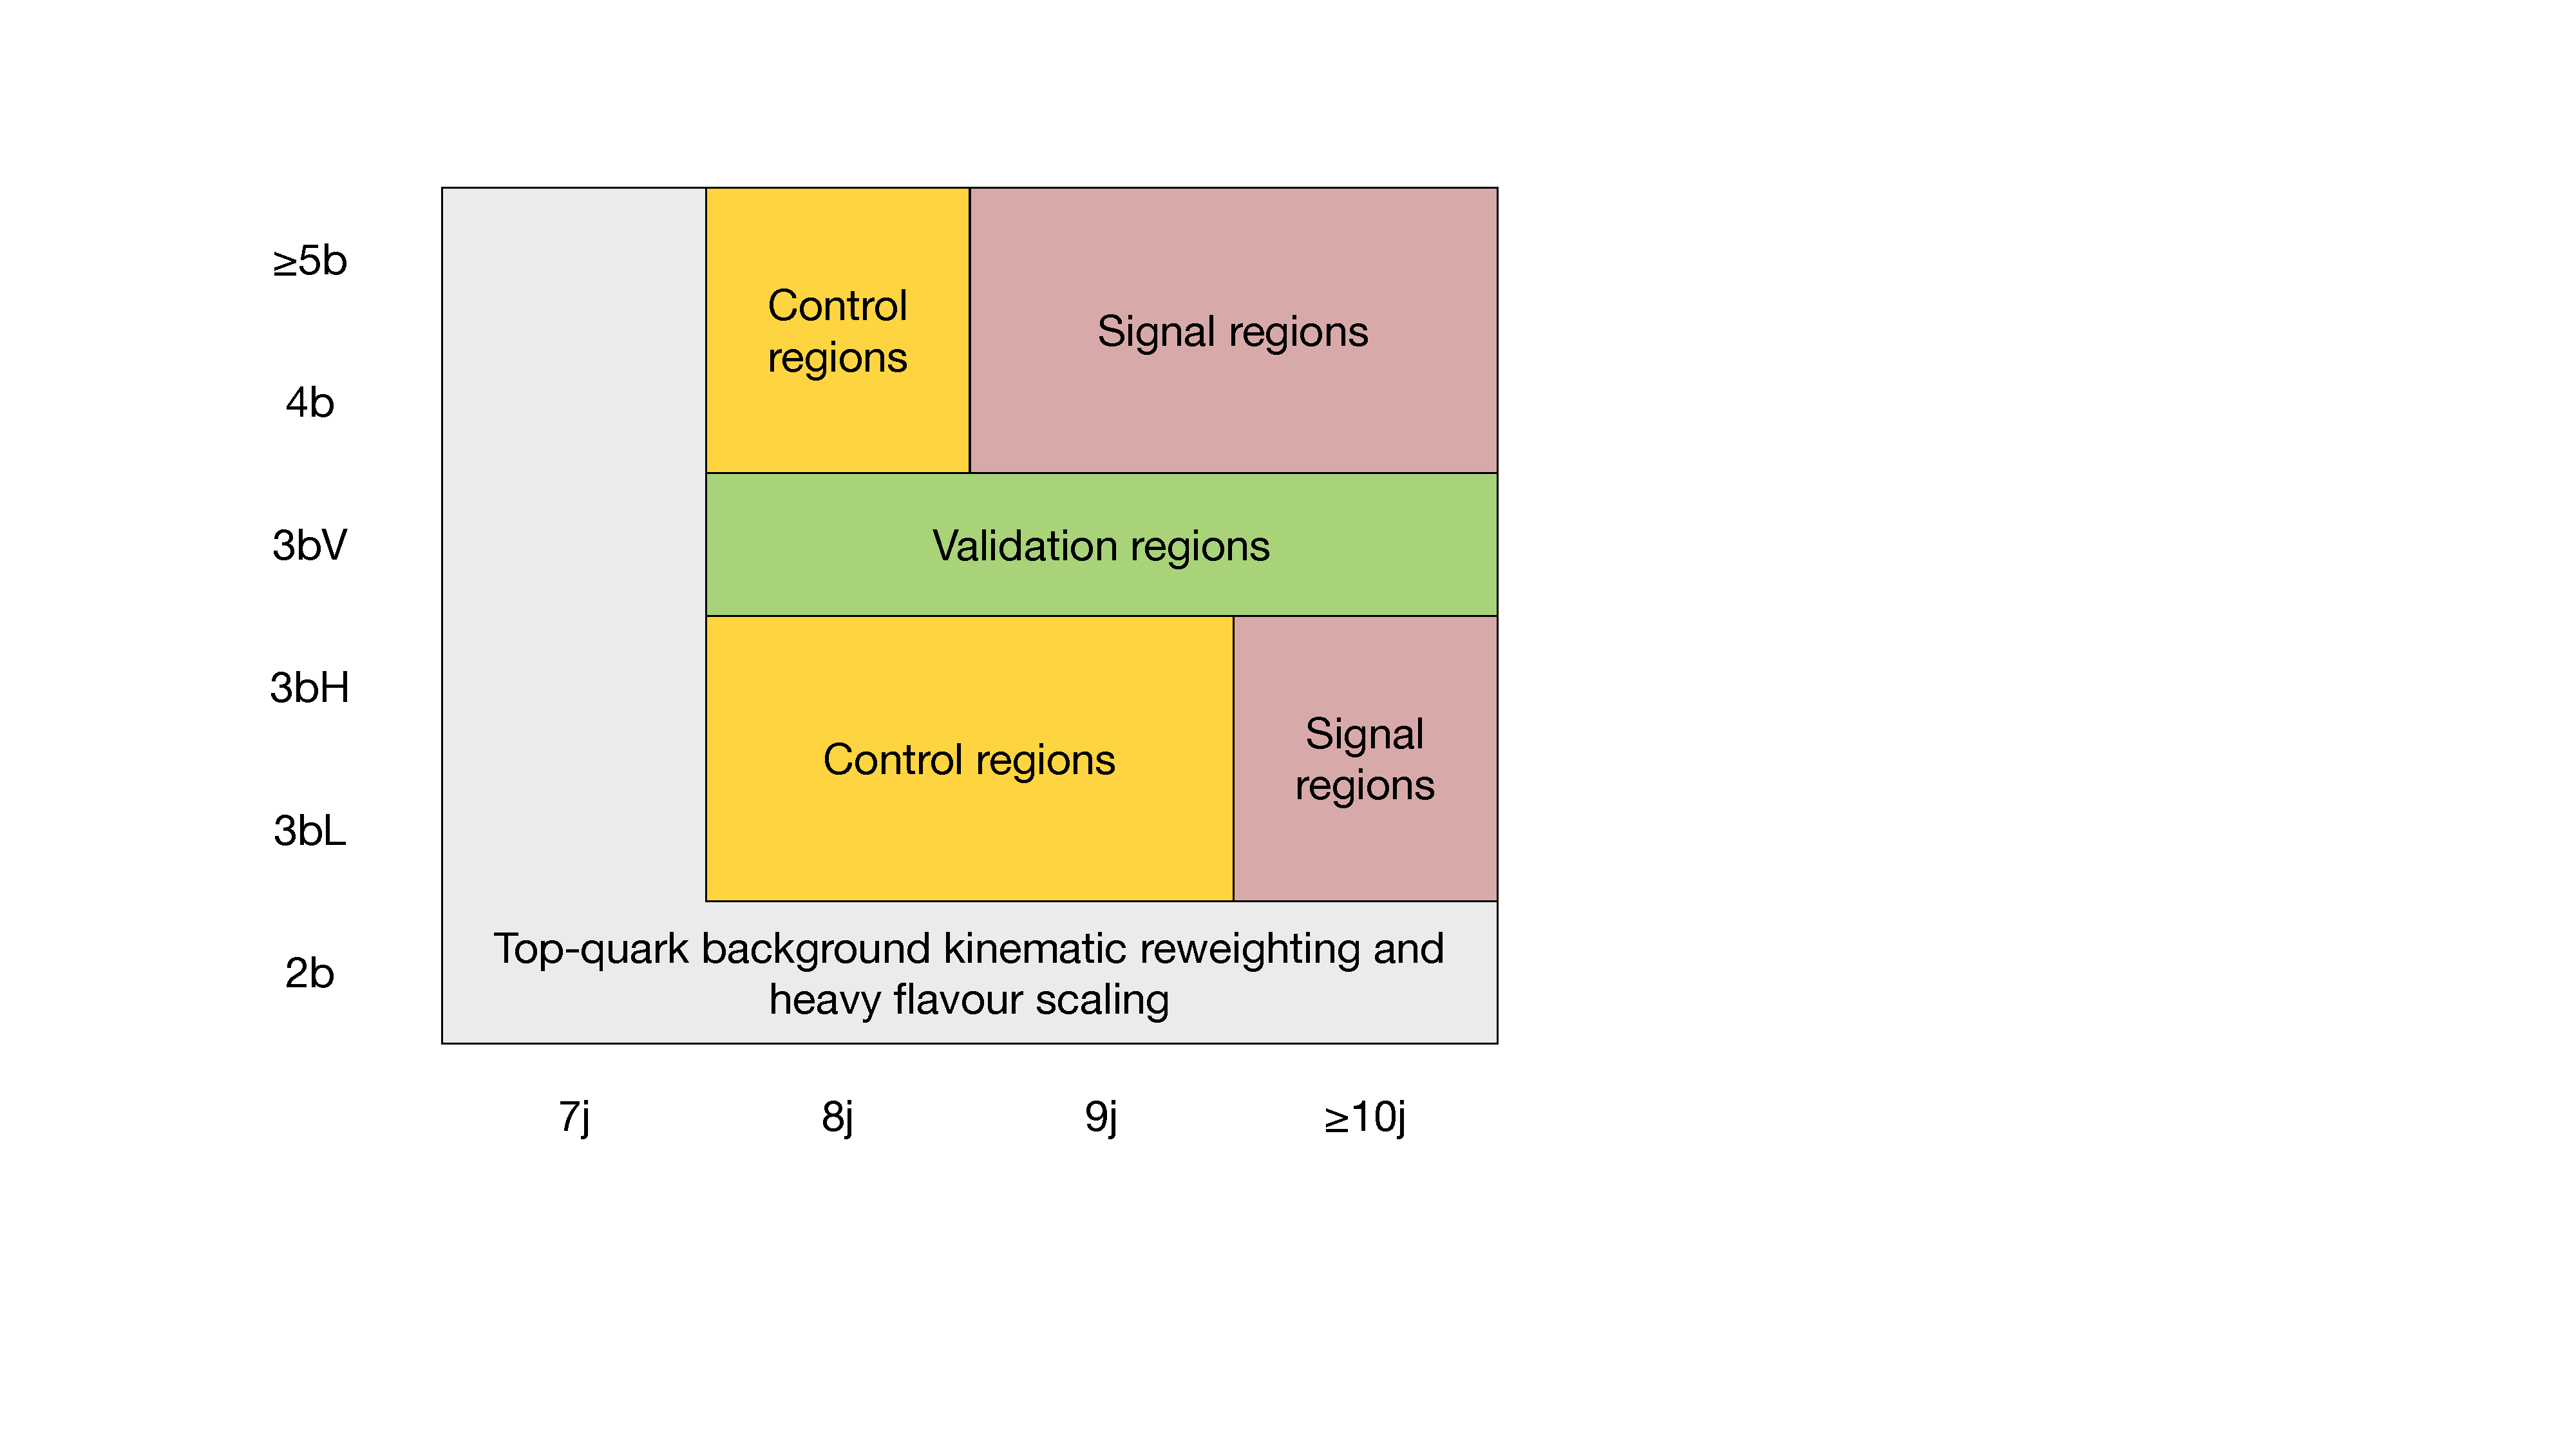
\includegraphics[width=0.46\textwidth]{figures/strategy/1l_regions} &
        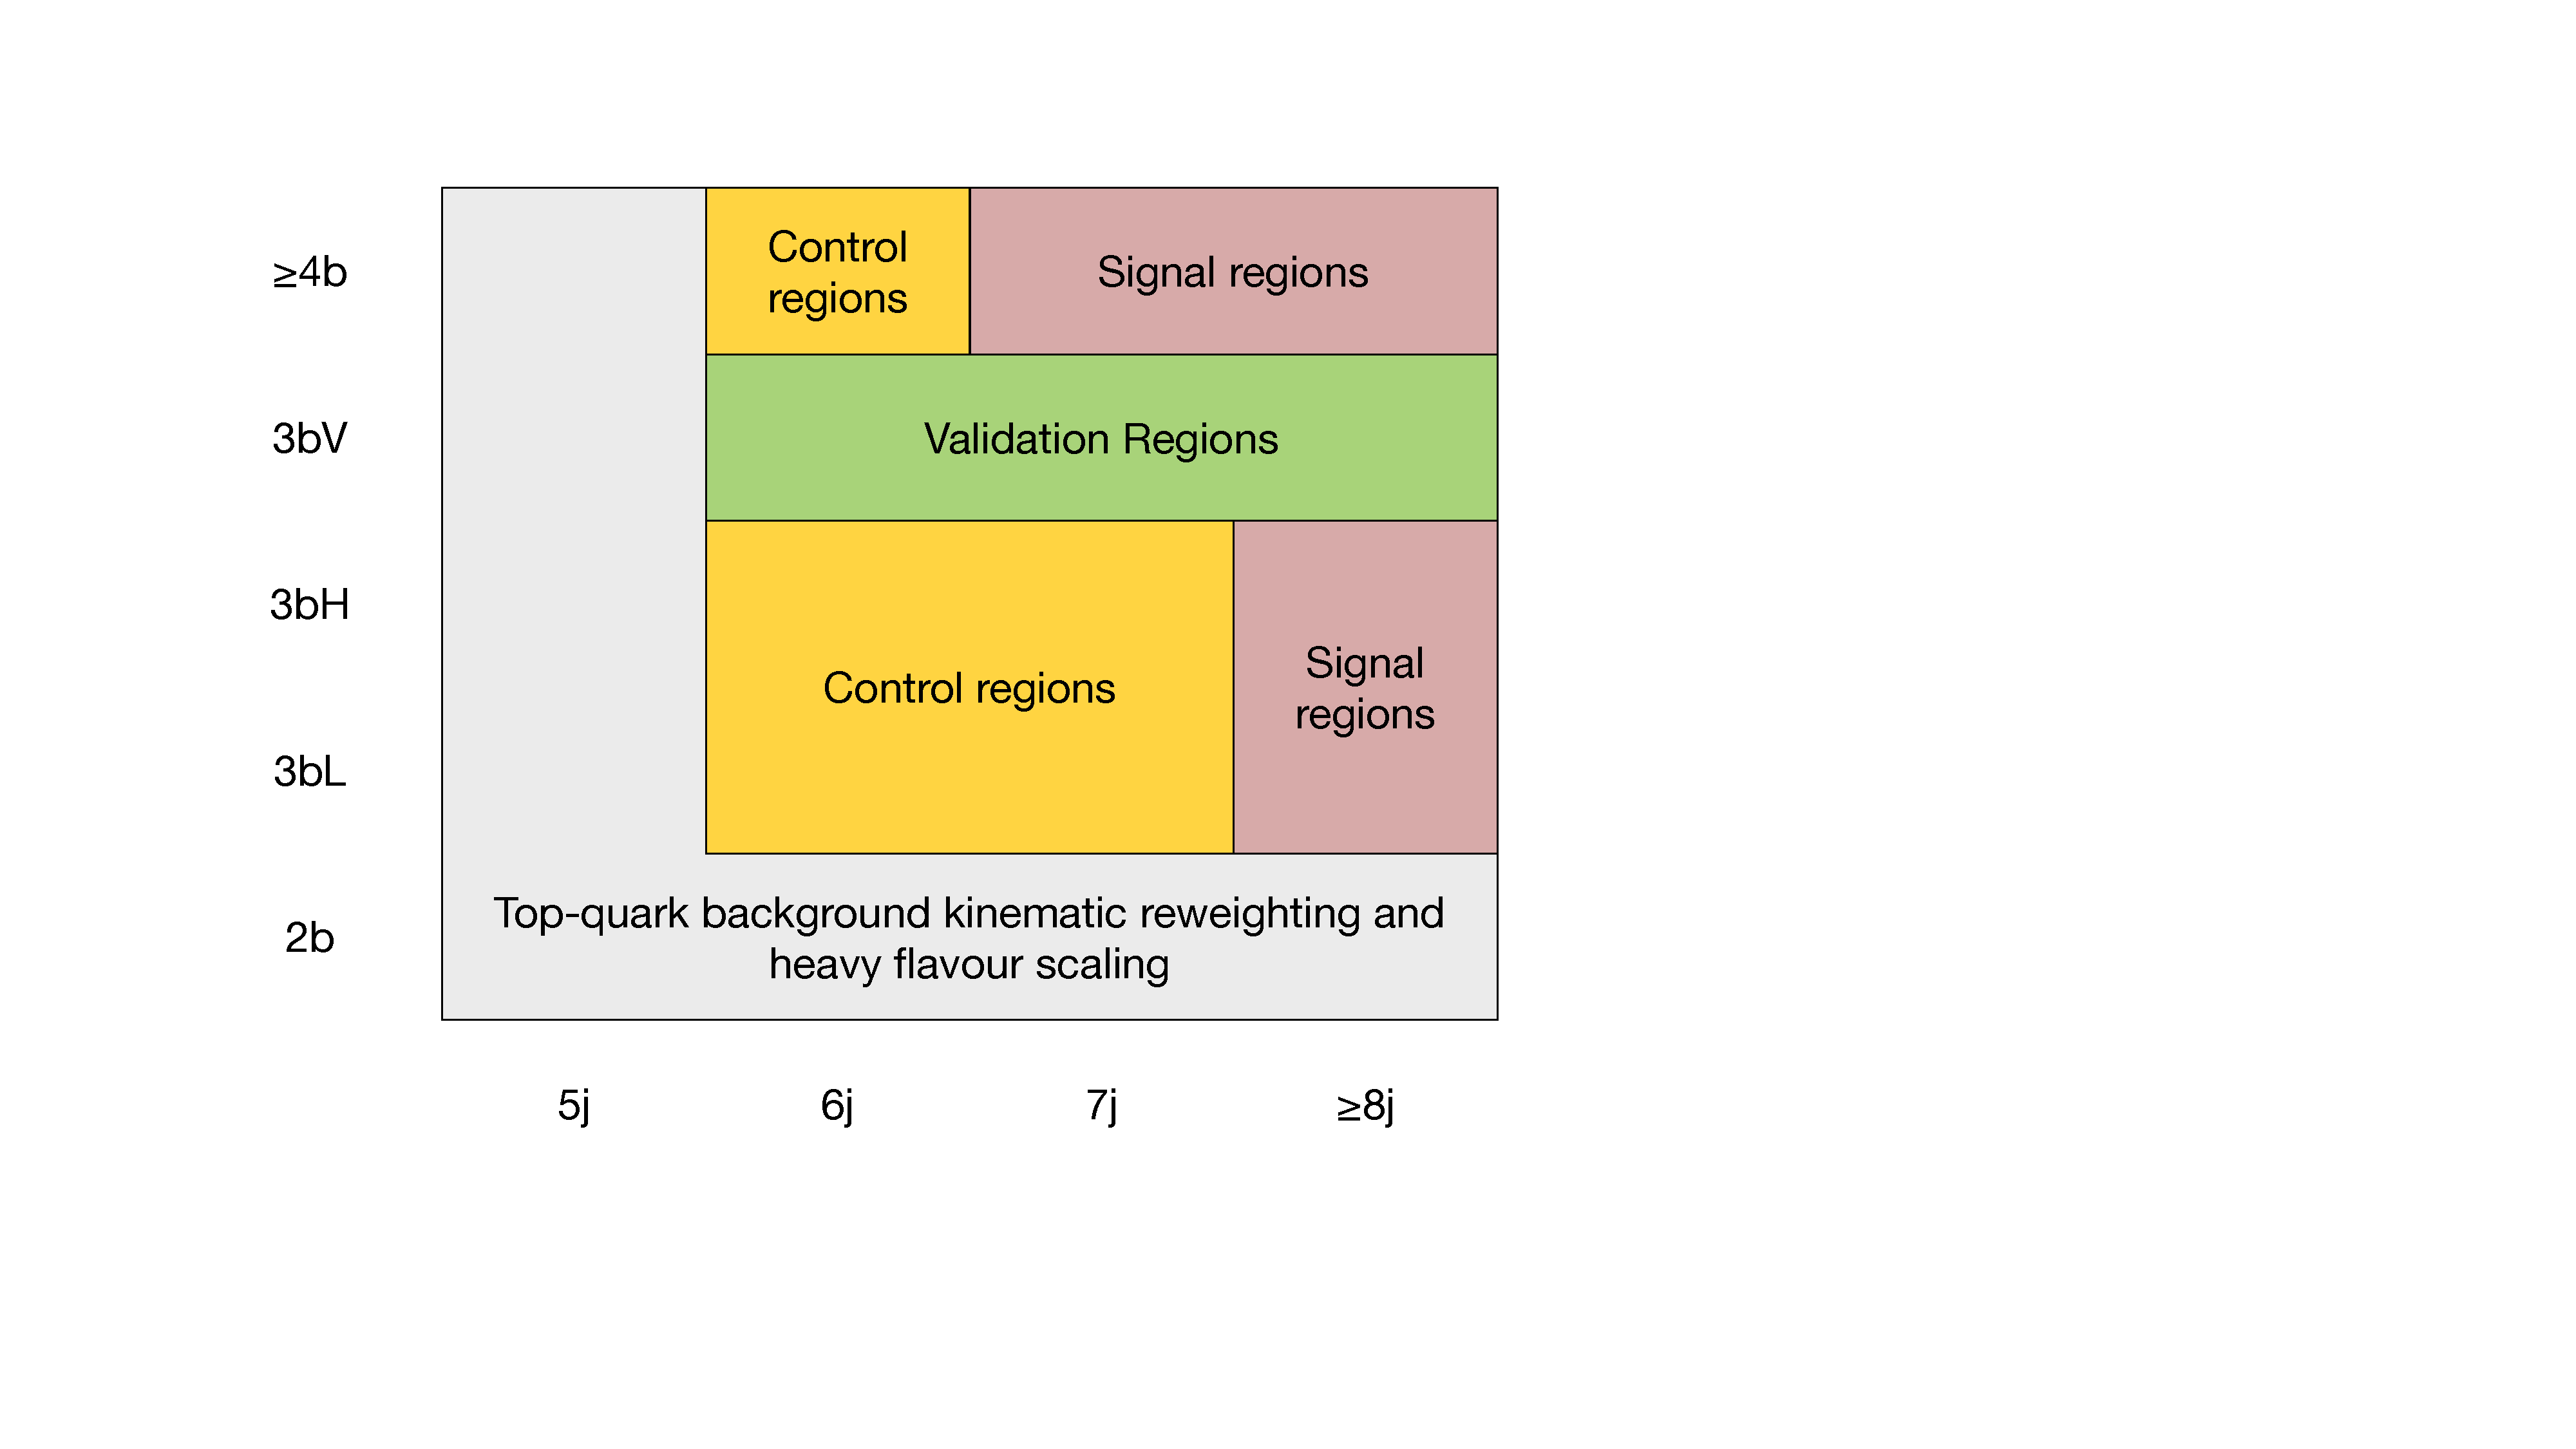
\includegraphics[width=0.46\textwidth]{figures/strategy/2los_regions} \\
        (1L) & (2LOS) \\
    \end{tabular}
     \caption{Schematic view of the event categories used to select analysis regions (signal, control, validation and $\ttbar$+jets reweighting regions) in the 1L channel (left) and 2LOS channel (right). The axes represent the jet multiplicity and $b$-tagging requirements defined in Table~\ref{tab:regions}. The 3bL (3bH) $b$-tagging requirement selects events with lower (higher) purity of MC 'truth' $b$-jets amongst the three jets tagged at the 70\% OP. The 3bV $b$-tagging requirement is used to define the validation regions.}
   \label{fig:regions}
  \end{center}
\end{figure}

The SM background is estimated by using samples of simulated events as described in Section~\ref{sec:samples}. 
The main background originates from $\ttbar$+jets production.  As discussed in Section~\ref{sec:nn_rew}, a reweighting procedure is implemented to adjust the MC modelling  of $\ttbar$+jets production based on a  combined use of events with low jet multiplicity and large b-jets multiplicity as well as events with large jet multiplicity and low b-jets multiplicity after checking that the signal contamination in those regions is negligible. The regions used to derive the reweighting for the $\ttbar$+jets background are highlighted in grey colour in Figure~\ref{fig:regions}. 

A potential BSM signal is identified by using MVA discriminants. As described in Section~\ref{sec:mva} two MVA discriminants are developed, are used throughout the analysis and facilitate their mutual validation by extensive fit studies and modelling studies in signal-depleted regions.    
The MVA and H$_T$ distributions from each of the regions with at least 3 $b$-jets are simultaneously used to test for the presence of a signal. 
A total of 21 regions are used in the profile likelihood fit, with 12 regions in the 1L channel and
9 regions in the 2LOS channel.
They are defined by considering the regions with at least 8 (6) jets in the 1L (2LOS) channel and
satisfying the 3bL, 3bH or $\ge$4b requirements.
Among these regions, the ones that have at least 10 (8) jets or have 9 (7) jets and satisfy the $\ge$4b
requirement in the 1L (2LOS) channel are defined as the signal regions.
The rest of the fitted regions are defined as the control regions.
A total of 6 validation regions are also defined by considering the regions with at least 8 (6)
jets in the 1L (2LOS) channel and satisfying the 3bV requirement.
The validation regions are not used in the fit and hence do not contribute to the signal extraction.
The variables and binning used in each region is optimised as discussed in Sec.~\ref{sec:binning}. 
